\begin{figure}[tb]
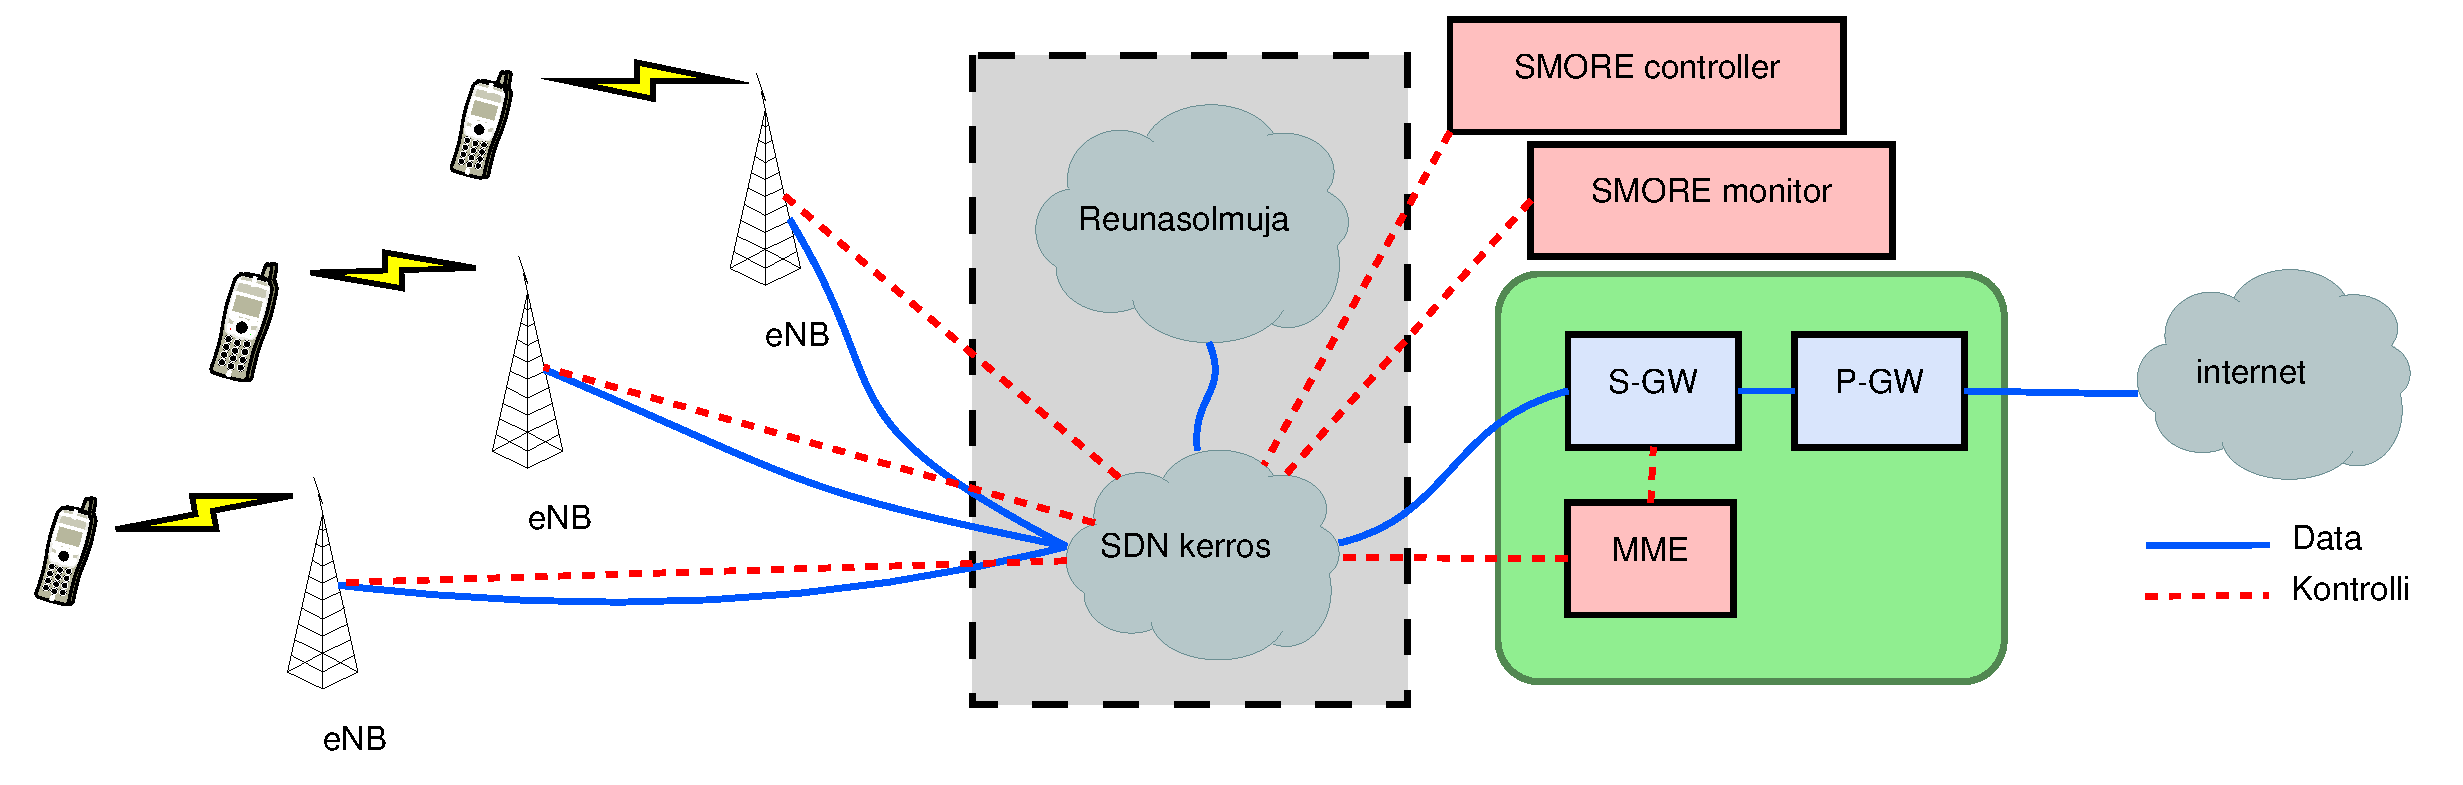
\includegraphics[width = \textwidth]{SMORE.eps}
\caption{Yksittäinen SMORE instanssi kuvattuna. Välissä sijaitseva harmaa alue kuvaa reunajärjestelmän sijaintia.} \label{fig:smore}
\end{figure}

\subsection{SMORE ja MobiScud} \label{smore}
SMORE (Software defined network Mobile Offloading aRchitecturE) on mobiiliverkkoihin suunnattu reunalaskentaratkaisu \cite{cho2014smore}.
Keskeisin osa ratkaisua on SDN käyttöönotto mobiiliverkon sisäisissä yhteyksissä.
SMORE:n tapauksessa reunajärjestelmä sijoittuu eNodeB ja S-GW välille. 

Ratkaisun kantavana ideana on SDN kerros. Se sijaitsee alkuperäisen idean mukaan MTSO:ssa (Mobile Telephone Switching Office), joka on tukiasemien kokoumapiste.
SDN kerroksessa sijaitsee SMORE monitor, joka tarkkailee SDN kerroksen läpi kulkevaa kontrollikerroksen liikennettä. SMORE monitor poimii tietoliikenteestä kontrollikerroksella esiintyviä tunnisteita kuten IMSI (International Mobile Subscriber Identity) ja GTP tunneleiden TEID tunnisteita. Nämä tunnisteet tallennetaan tietokantaan.
SMORE controller on vastuussa reunasovelluksien käynnistämisestä sekä SDN reitityssääntöjen päivittämisestä. SMORE controller voi tietokantaan tallennettujen tietojen perusteella muokata reitityssääntöjä siten että asiakkaan tietoliikenne ohjautuu reunasolmuille. 

Varsinainen tietoliikenteen haarauttaminen tehdään virtuaalisten porttien avulla jotka tarkkailevan GTP pakettien kohte IP-osoitteita. Mikäli kohde IP on reunasolmu virtuaalisen portin sisällä oleva toiminnallisuus purkaa GTP tunneloinnin ja ohjaa paketin reunasolmulle. Reunasolmulta asiakaslaitteelle suuntautuva liikenne hoituu siten että SMORE monitorin poimimista tiedoista saadaan asiakaslaitteen IP-osoitetta vastaava GTP TEID.
Tämän avulla SDN kerroksessa voidaan suorittaa GTP paketointi ja paketti voidaan välittää normaalin toiminnallisuuden mukaisesti mobiiliverkossa. 

SMORE controllerin vastuulle kuuluu myös reunasolmujen tarjoamien palveluiden hallinnointi. SMORE:n esittelyn yhteydessä laukaisumekanismiksi esitettiin....,

Koska SDN kerros ei koske mobiiliverkon kontrollikerrokseen tai muuhun  internettiin suuntautuvaan tietoliikenteeseen järjestelmä on asiakaslaitteen ja mobiiliverkon näkökulmasta näkymätön.


SDN käyttöönotolla tavoitellaan sitä, että televerkon toimintaan ei tarvitsisi tehdä muutoksia. Minkään olemassa olevan komponentin toiminta ei siis muutu. 
SMORE:n toiminta on jaettu kahteen osaa, joita varten SDN on käytössä. 
Ensimmäisenä on mobiiliverkon kontrollitasolla (control-plane) tapahtuva viestien monitorointi. 
Toisena toimintona on monitoroitujen tietojen pohjalta tehtävät SDN hallintatoimenpiteet. Näiden avulla voidaan ohjata haluttu osa tietoliikenteestä haluttuihin reunalaskentayksikköihin.
Kontrollitasolla viestejä monitorointia suorittaa SMORE monitori (SMORE monitor) ja tietoliikenteen ohjauspäätöksistä vastaava komponentti on SMORE kontrolleri (SMORE controller).

Tietojen välitys SMORE kontrollerin ja SMORE monitorin välillä on toteutettu yhteisen tietokannan kautta. SMORE monitor tallentaa poimitut tiedot tietokantaan ja antaa tiettyjen tapahtumien yhteydessä SMORE kontrollerille herätteen tehdä asianmukaiset muutokset SMORE:n SDN reitityksiin. Herätteitä laukaisevat tapahtumat ovat asikkaan liittyminen verkkoon ja asikkaan liikkuminen verkossa.

SMORE monitori tarkkailee asiakaslaitteen ja LTE/EPC:n välistä liikennettä.
Asiakaslaitteen liittyessä mobiiliverkkoon, asiakaslaite ja LTE/EPC:n sisäiset komponenti muodostavat tunneleita ja asiakaslaitteeseen liitetään erilaisia tunneleita koskevia osoite ja metatietoja.
SMORE monitorin tehtävänä on poimia asiakaslaitteen liittyessä ja yhteydenmuodostuksen aikana asiakaslaitteisiin liittyviä tietoja.
Asiakaslaitteen lähettäessä liittymispyynnön (attach request) SMORE monitori poimii pyynnöstä asiakaslaitteen IMSI (international Mobile Subscriber Identity) ja TAI:n (Tracking Area Identifier). 
Tämän jälkeen SMORE monitori poimii MME:n asiakaslaitteelle lähettämästä liittymispyynnön hyväksymis -viestistä (attach accept) monitori poimii asiakaslaitteelle annetun IP-osoitteen, SGW:n IP-osoitteen, SGW:n TEID:n ja asiakaslaitteen GUTI:n (Globally Unique Temporary Id).
Tämän jälkeen eNodeB neuvottelee asiakaslaitteen kanssa radioyhteydestä ja tämän lopputulos välitetään MME:lle. SMORE monitor poimii eNodeB:n ja MME:n välisestä kommunikaatiosta eNodeB:n IP-osoitteen ja eNodeB:n TEID:n.
Kun edellä mainitut tiedot on tallennettu SMORE:n tietokantaan, SMORE monitor lähettää SMORE kontrollerille herätteen päivittää SDN reitityksiä. 

Toinen tapahtuma josta SMORE kontrolleri on kiinnostunut on handover, eli mikäli asiakaslaite siirtyy mobiiliverkossa eNodeB:den välillä. SMORE kontrollerin on tässä tapauksessa kiinnostunut mobiiliverkossa tapahtuvista muutoksista. 
Handover alkaa kun tällä hetkellä käytössä oleva eNodeB päättää, että on aika siirtää asiakaslaitteen yhteys toiselle eNodeB:lle (kohde).
Alkuperäinen eNodeB välittää pyynnön kohteena olevalle eNodeB:lle joka oletettavasti hyväksyy sen. Tämän jälkeen, kohteena oleva eNodeB pyytää MME:ltä reitityksen muutosta. Tässä välissä oleva SMORE monitor poimii reitityksen muutosta koskevan tiedon ja välittää ne SMORE kontrollerille.
Tämän tiedon pohjalta SMORE kontroller voi tehdä SDN muutokset siten että vanhat reititykset voidaan poistaa ja korvata uusilla.


\subsubsection{MobiScud} \label{mobiscud}
MobiScud \cite{wang2015mobiscud} on SMORE:n ideoita ammentava versio reunalaskentapalveluiden tuottamisesta mobiiliverkoissa.
MobiScud:in perustoiminnallisuus on hyvin samankaltainen kuin SMORE:ssa. MobiScud painottaa enemmän käyttäjän tarvetta liikkua verkossa. Lisäksi MobiScud käyttää hyödykseen oletusta mobiiliverkkojen hajautettua rakennetta. 

Kuten SMORE, MobiScud käyttää hyödykseen SDN:n tarjoamia ominaisuuksia ja siten olettaa sen käyttöönottoa palveluntarjoajan infrastruktuurissa. Lisäksi MobiScudin toiminnallisuudet on ajateltu toteutettavan Network Function Virtualisantionin (NFV) avulla. 
MobiScud Controller (MC) koostuu kahdesta loogisesta kokonaisuudesta: monitorista ja kontrollerista. Näiden toimintaperiaate on käytännössä identtinen SMORE:n vastaavan nimisiin toimijoihin. MC:n sijaintia ei kuitenkaan ole keskitetty kuten SMORE:ssa vaan sen oletetaan sijaitsevan hajautettna RAN ja EPC välissä.
Käyttäjän ja reuna-infrastruktuurin välinen yhteys toteutetaan hyvin samalla tavalla kuin SMORE:ssa. 

MobiScudin reunapalvelut on ajateltu toteutettavan hyvin cloudletmäisesti. Mahdollisimman lähellä reunaa sijaitsevassa "pilvessä" on palvelinresursseja, joita käyttäjät hyödyntävät yksityisien virtuaalikoneinstanssien muodossa (Private Virtual Machinem, PVM). 

MobiScudin tavoitteena on tarjota asiakkaalle mahdollisimman nopea yhteys asiakkaan ja PVM:n välille. MobiScud hyödyntää televerkon omia kontrollitason viestejä asiakkaan liikkumisen seuraamiseen. Kun handoverista tulee viesti MC:n monitoroivalle entiteetille, alkaa MC organisoimaan reunalaskentaan liittyviä muutoksia. 

Asiakkaan siirtyessä tukiasemalta toiselle PVM:n siirto aloitetaan livemigraationa kohteena olevalle "pilvelle". Livemigraation ollessa käynnissä kohteena olevan pilven MC huolehtii että asiakaslaitteella on edelleen yhteys alkuperäiseen sijaintiinsa. Tämä hoidentaan SDN reititysmuutoksilla. Kun PVM:n livemigraatio on saatu suoritettua alkuperäisen sijainnin MC ilmoittaa tästä kohdesijainnin MC:lle, joka puolestaa päivittää SDN reititykset ohjaamaan siirretylle PVM:lle.

MobiScudin testeissä livemigraation ja SDN reitityksien avulla RTT (round trip time) saatiin pidettyä pienenä. Kuitenkin yhteyksissä aiheutui noin kahden sekunnin mittaisia katkoksia sillä hetkellä kun livemigraation viimeiset muutokset lähetetään. Yhteyskatkoksen pituuteen vaikuttavat monet asiat ja artikkelissa huomautetaankin että nykyinen toteutus oli optimoimaton ja vaatii jatkotutkimuksia.

